\section{Observations}
% description of apparatus, settings objects, exposure times, weather, calibration, etc

This experiment is performed with the {\it Stony Brook Michelson Radio Interferometer} \cite{sbu},  during the mornings of February 17th and 26th of 2012. The {\it geographic coordinates} of the site  where we were to performed the observations are  $40^o 54'$ N  $73^o 08'$ W. 

The interferometry data was taken only on the second day, from 10 a.m. until 13 p.m (Eastern Standard Time). The weather was reported as sunny, with temperature around $7^o$C, and NW winds up to 15 km/h. The altitude and azimuth coordinates of the Sun for the day of the observation are shown  in the appendix, in the table \ref{a-sun}.



The Stony Brook's radio interferometer consists of an electronic part, named {\it Detector}, and a mechanic  part, named {\it Radiotelescope}, which is further divided ona mount and  the drive. 




\bigskip

\subsection{The Radiotelescope}\label{radio_interferometer}
The radiotelescope is a dish on a base attached to a frontal ladder. Conceptually it can subdivided on the following parts (also illustrated in the figure \ref{2-sketch}):
\begin{description}
\item [Siderostat:] A central and two lateral mirrored pieces, where the two last have  variable distance lengths (the different  {\it baseline lengths} in this experiment). The siderostat combines light onto a single target. The reflective element was building with aluminum foils (reflectivity of 96$\%$  \cite{sbu}), appropriated to radio observations, \eg centimeter wavelengths  in this case. 

\item [Satellite Dish:] Located to be pointed to the target. In the case of the {\it single dish radio observations}, it will be pointed directly to the source (flipped $180^o$ from the mirrors), \ie pointing to the opposite side of the siderostats. In the case of the interferometry observations,  the central mirror is faced to the the satellite dish antenna, and this  will vectorially add the electromagnetic signals received from the source by the two side side mirrors. The broadcast satellite dish operates with frequency/wavelength $\nu \sim 11 \mbox{ GHz, } \lambda \sim 2.7 \mbox{ cm}$ \cite{sbu}. 

\item [Adjustable Baseline Length:] A rail designed on a man-hold  ladder, where the left and the right pieces of the siderostat slide, allowing different  baseline lengths. 

\item [Mount:] Driven with motors that electronically adjusts azimuth (left - right) and elevation (up - down), covering 180 degrees.
\end{description}



 \begin{figure}[htb]
\begin{center}
 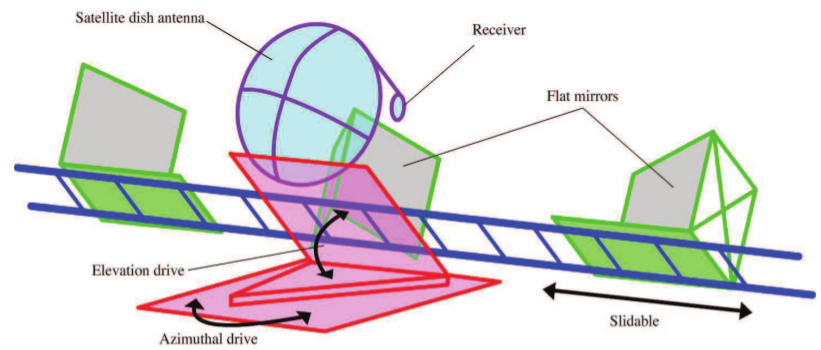
\includegraphics[scale=0.5]{figs/1.png}
\caption{Pictorial illustration of the Stony Brook's Michelson-type radio interferometer: the mirrors  can slide through the rail for adjustable baseline lengths. The Central dish stays on front of the satellite dish antenna. }
\label{2-sketch}
\end{center}
\end{figure}


\bigskip


\subsection{The Detection and Analysis Systems}\label{detection_system}

The electronic part of the experiment is composed of commercial receiver amplifier (satellite finder)  and analog-to-digital converter (labpro) connected to a computer \cite{sbu}. The output is given in voltage (volt) by time (seconds), and acquired in the computer through the software {\it LoggerPro} \cite{loggerpro}. To convert the observed spectra to {\it power response}, we use the specified {\it Voltage (V) versus Power(dBm) curve}, figure \ref{conv}, in the appendix. The slope is reported as  $s = - 25(mV/dB),$ resulting on
\begin{equation}
P_{dBm} (t)  = \frac{u(t) \mbox{ V}}{(-25 \mbox{ mV})},
\label{pdb}
\end{equation}
with the conversion of {\it decibel m} into a linear power scale is
\begin{equation}
P (t)  = 10^{\frac{P_{dBm}(t) - 30}{10}}.
\label{pdb2}
\end{equation}




\bigskip

\subsection{Methodology of the Observations}\label{observations}

After the initial calibration (subsection \ref{calibration}), we proceeded with the data acquisition, which is divided on four parts:

\begin{enumerate}
 \item {\bf Satellite's Single Dish Response}: After positioning the receiver directly the coordinates of of a point source, \eg a geostationary TV satellite, we performed two scans of the power response  for the  single dish, with $\Delta \theta^{single}_{4,5} = 10^o$, varying azimuthally.

 \item {\bf Sun's Single Dish Response}:After positioning the receiver directly to the Sun (azimuth and elevation showed in the table \ref{a-sun}), we performed three scans of its power response, with $\Delta \theta^{sin}_{1,2,3} = 15^o$, varying azimuthally. From this measurement, and normalizing with the previous satellite's measurements, we marginally infer the Sun's angular diameter, $\Phi_{sun}^{Sin}$.

 \item {\bf Sun's Interferometer Response}: The receiver is  faced to the interferometer central mirror, and, after calibration, we performed five scans of the power response of the Sun, with five different baselines lengths,  $B^{meas}_{1,2,3,4,5}$, and  with $\Delta \theta^{sun}_{1,2,3,4,5} = 20^o$.

 \item {\bf Satellite Source's Interferometer Response}: We performed five scans of the power response of the point source, with the same five different baseline lengths, $B^{meas}_{1,2,3,4,}5$, and  with $\Delta \theta^{sat}_{1,2,3,4,5} = 10^o$.
\end{enumerate}


\bigskip


\subsection{Methodology of the Calibration}\label{calibration}

The calibration of the radiotelescope was performed in the following way:
\begin{description}
 \item [Calibrating the azimuth disk and the elevation dial with Sun]  We need this to minimize the effect of the telescope aperture attenuation on the measurement of $P_{max}$ and $P_{min}$ (equation (\ref{vis})) when we measure the Sun. In another words, the central maximum of the interference pattern should be $\theta = \theta_0$ of the source. With the correct position of the Sun (table \ref{a-sun}) we point the single dish detector directly to it and, together with an analogical Satellite Finder and the LoggerPro software, we find the position with highest intensity, scanning vertically. We then trail the elevation dial to the corrected aligned. We use the latter shadow to align the sun (looking to its shadow) and the azimuth disk can be calibrated.

\item [Calibrating the Mirrors] For the {\it Interferometry} observation, we rotate the dish to the center of the central mirror, with the left and right mirror on their closest position from the center. We maximize the signal by refining the aim of the telescope. First, measuring the power for the left mirror alone. Then, performing the measurement with the right mirror alone. We verifies how the reflected intensities matches. 
\end{description}

 
\bigskip





